\documentclass[1p]{elsarticle_modified}
%\bibliographystyle{elsarticle-num}

%\usepackage[colorlinks]{hyperref}
%\usepackage{abbrmath_seonhwa} %\Abb, \Ascr, \Acal ,\Abf, \Afrak
\usepackage{amsfonts}
\usepackage{amssymb}
\usepackage{amsmath}
\usepackage{amsthm}
\usepackage{scalefnt}
\usepackage{amsbsy}
\usepackage{kotex}
\usepackage{caption}
\usepackage{subfig}
\usepackage{color}
\usepackage{graphicx}
\usepackage{xcolor} %% white, black, red, green, blue, cyan, magenta, yellow
\usepackage{float}
\usepackage{setspace}
\usepackage{hyperref}

\usepackage{tikz}
\usetikzlibrary{arrows}

\usepackage{multirow}
\usepackage{array} % fixed length table
\usepackage{hhline}

%%%%%%%%%%%%%%%%%%%%%
\makeatletter
\renewcommand*\env@matrix[1][\arraystretch]{%
	\edef\arraystretch{#1}%
	\hskip -\arraycolsep
	\let\@ifnextchar\new@ifnextchar
	\array{*\c@MaxMatrixCols c}}
\makeatother %https://tex.stackexchange.com/questions/14071/how-can-i-increase-the-line-spacing-in-a-matrix
%%%%%%%%%%%%%%%

\usepackage[normalem]{ulem}

\newcommand{\msout}[1]{\ifmmode\text{\sout{\ensuremath{#1}}}\else\sout{#1}\fi}
%SOURCE: \msout is \stkout macro in https://tex.stackexchange.com/questions/20609/strikeout-in-math-mode

\newcommand{\cancel}[1]{
	\ifmmode
	{\color{red}\msout{#1}}
	\else
	{\color{red}\sout{#1}}
	\fi
}

\newcommand{\add}[1]{
	{\color{blue}\uwave{#1}}
}

\newcommand{\replace}[2]{
	\ifmmode
	{\color{red}\msout{#1}}{\color{blue}\uwave{#2}}
	\else
	{\color{red}\sout{#1}}{\color{blue}\uwave{#2}}
	\fi
}

\newcommand{\Sol}{\mathcal{S}} %segment
\newcommand{\D}{D} %diagram
\newcommand{\A}{\mathcal{A}} %arc


%%%%%%%%%%%%%%%%%%%%%%%%%%%%%5 test

\def\sl{\operatorname{\textup{SL}}(2,\Cbb)}
\def\psl{\operatorname{\textup{PSL}}(2,\Cbb)}
\def\quan{\mkern 1mu \triangleright \mkern 1mu}

\theoremstyle{definition}
\newtheorem{thm}{Theorem}[section]
\newtheorem{prop}[thm]{Proposition}
\newtheorem{lem}[thm]{Lemma}
\newtheorem{ques}[thm]{Question}
\newtheorem{cor}[thm]{Corollary}
\newtheorem{defn}[thm]{Definition}
\newtheorem{exam}[thm]{Example}
\newtheorem{rmk}[thm]{Remark}
\newtheorem{alg}[thm]{Algorithm}

\newcommand{\I}{\sqrt{-1}}
\begin{document}

%\begin{frontmatter}
%
%\title{Boundary parabolic representations of knots up to 8 crossings}
%
%%% Group authors per affiliation:
%\author{Yunhi Cho} 
%\address{Department of Mathematics, University of Seoul, Seoul, Korea}
%\ead{yhcho@uos.ac.kr}
%
%
%\author{Seonhwa Kim} %\fnref{s_kim}}
%\address{Center for Geometry and Physics, Institute for Basic Science, Pohang, 37673, Korea}
%\ead{ryeona17@ibs.re.kr}
%
%\author{Hyuk Kim}
%\address{Department of Mathematical Sciences, Seoul National University, Seoul 08826, Korea}
%\ead{hyukkim@snu.ac.kr}
%
%\author{Seokbeom Yoon}
%\address{Department of Mathematical Sciences, Seoul National University, Seoul, 08826,  Korea}
%\ead{sbyoon15@snu.ac.kr}
%
%\begin{abstract}
%We find all boundary parabolic representation of knots up to 8 crossings.
%
%\end{abstract}
%\begin{keyword}
%    \MSC[2010] 57M25 
%\end{keyword}
%
%\end{frontmatter}

%\linenumbers
%\tableofcontents
%
\newcommand\colored[1]{\textcolor{white}{\rule[-0.35ex]{0.8em}{1.4ex}}\kern-0.8em\color{red} #1}%
%\newcommand\colored[1]{\textcolor{white}{ #1}\kern-2.17ex	\textcolor{white}{ #1}\kern-1.81ex	\textcolor{white}{ #1}\kern-2.15ex\color{red}#1	}

{\Large $\underline{12a_{0774}~(K12a_{0774})}$}

\setlength{\tabcolsep}{10pt}
\renewcommand{\arraystretch}{1.6}
\vspace{1cm}\begin{tabular}{m{100pt}>{\centering\arraybackslash}m{274pt}}
\multirow{5}{120pt}{
	\centering
	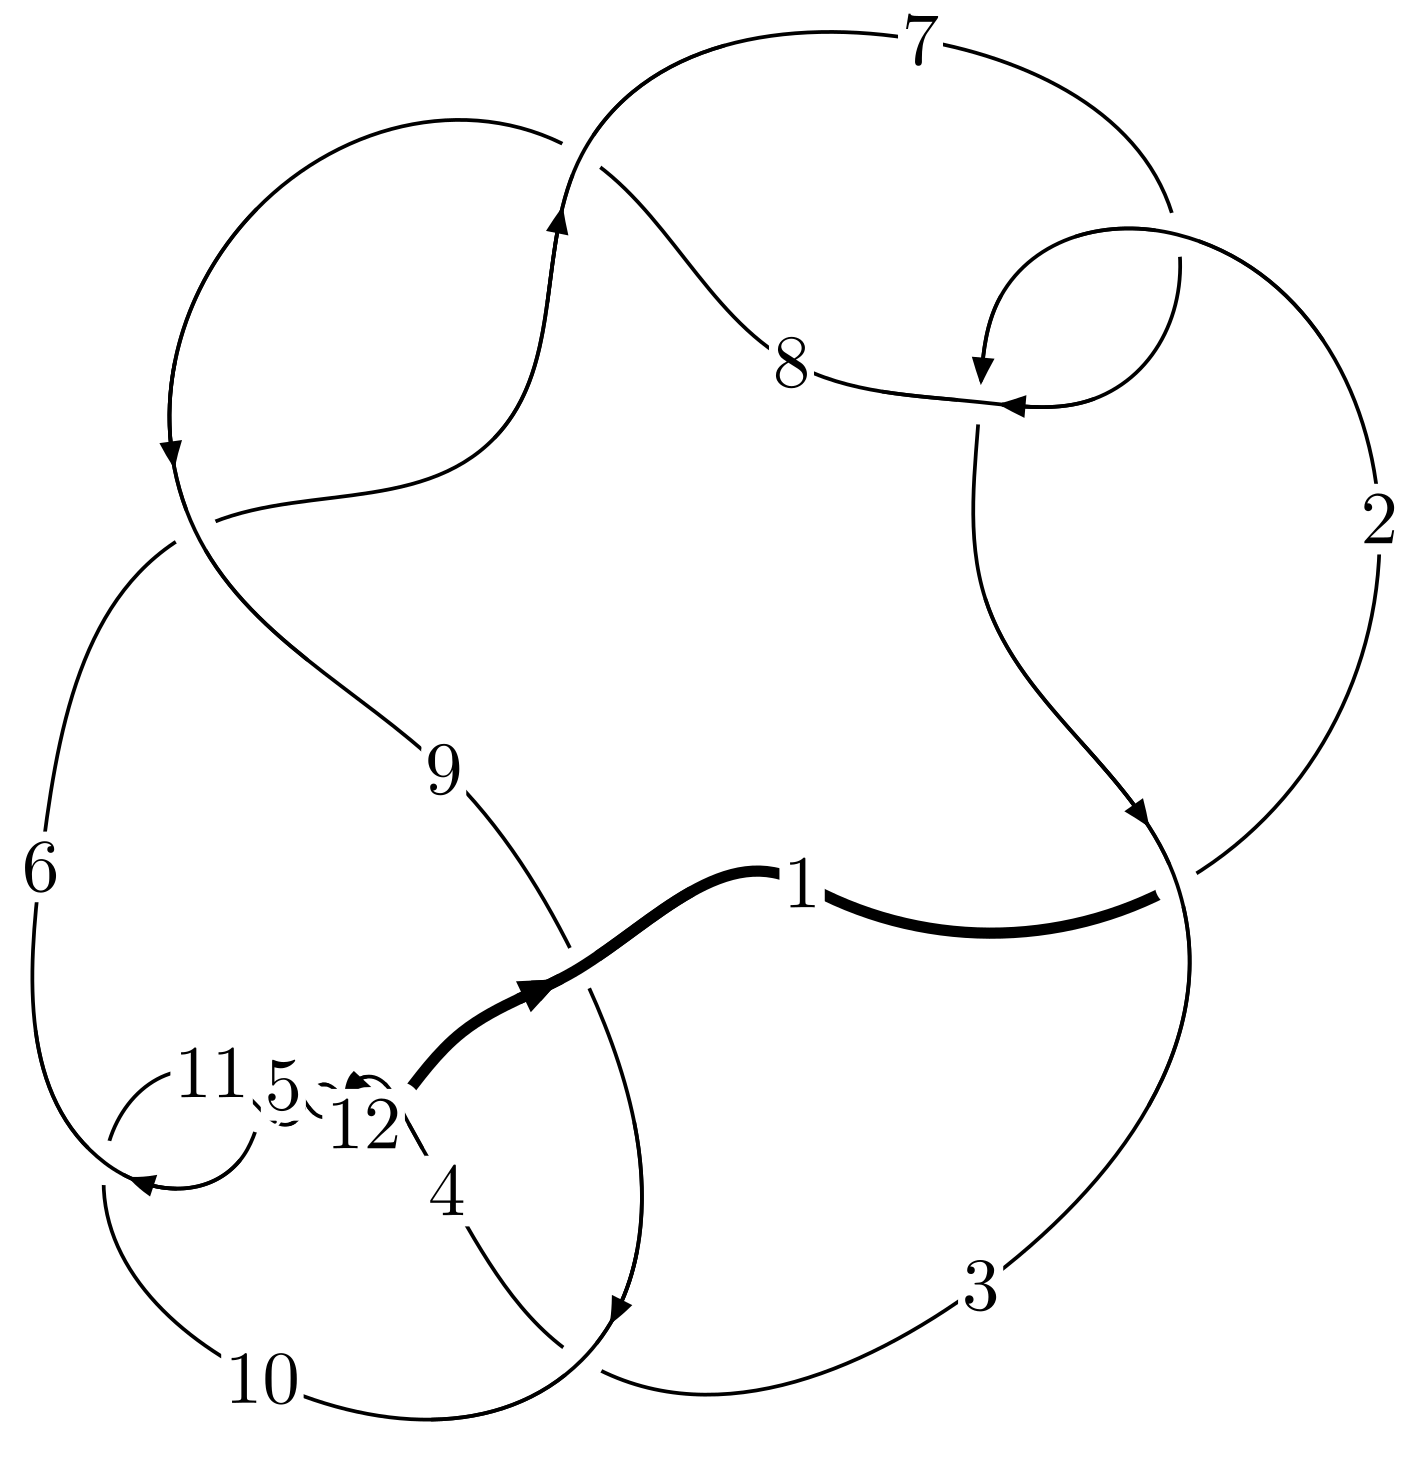
\includegraphics[width=112pt]{../../../GIT/diagram.site/Diagrams/png/1575_12a_0774.png}\\
\ \ \ A knot diagram\footnotemark}&
\allowdisplaybreaks
\textbf{Linearized knot diagam} \\
\cline{2-2}
 &
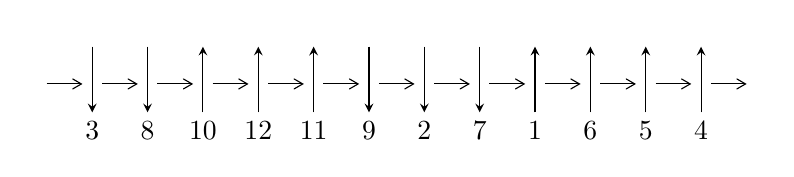
\begin{tikzpicture}[x=20pt, y=17pt]
	% nodes
	\node (C0) at (0, 0) {};
	\node (C1) at (1, 0) {};
	\node (C1U) at (1, +1) {};
	\node (C1D) at (1, -1) {3};

	\node (C2) at (2, 0) {};
	\node (C2U) at (2, +1) {};
	\node (C2D) at (2, -1) {8};

	\node (C3) at (3, 0) {};
	\node (C3U) at (3, +1) {};
	\node (C3D) at (3, -1) {10};

	\node (C4) at (4, 0) {};
	\node (C4U) at (4, +1) {};
	\node (C4D) at (4, -1) {12};

	\node (C5) at (5, 0) {};
	\node (C5U) at (5, +1) {};
	\node (C5D) at (5, -1) {11};

	\node (C6) at (6, 0) {};
	\node (C6U) at (6, +1) {};
	\node (C6D) at (6, -1) {9};

	\node (C7) at (7, 0) {};
	\node (C7U) at (7, +1) {};
	\node (C7D) at (7, -1) {2};

	\node (C8) at (8, 0) {};
	\node (C8U) at (8, +1) {};
	\node (C8D) at (8, -1) {7};

	\node (C9) at (9, 0) {};
	\node (C9U) at (9, +1) {};
	\node (C9D) at (9, -1) {1};

	\node (C10) at (10, 0) {};
	\node (C10U) at (10, +1) {};
	\node (C10D) at (10, -1) {6};

	\node (C11) at (11, 0) {};
	\node (C11U) at (11, +1) {};
	\node (C11D) at (11, -1) {5};

	\node (C12) at (12, 0) {};
	\node (C12U) at (12, +1) {};
	\node (C12D) at (12, -1) {4};
	\node (C13) at (13, 0) {};

	% arrows
	\draw[->,>={angle 60}]
	(C0) edge (C1) (C1) edge (C2) (C2) edge (C3) (C3) edge (C4) (C4) edge (C5) (C5) edge (C6) (C6) edge (C7) (C7) edge (C8) (C8) edge (C9) (C9) edge (C10) (C10) edge (C11) (C11) edge (C12) (C12) edge (C13) ;	\draw[->,>=stealth]
	(C1U) edge (C1D) (C2U) edge (C2D) (C3D) edge (C3U) (C4D) edge (C4U) (C5D) edge (C5U) (C6U) edge (C6D) (C7U) edge (C7D) (C8U) edge (C8D) (C9D) edge (C9U) (C10D) edge (C10U) (C11D) edge (C11U) (C12D) edge (C12U) ;
	\end{tikzpicture} \\
\hhline{~~} \\& 
\textbf{Solving Sequence} \\ \cline{2-2} 
 &
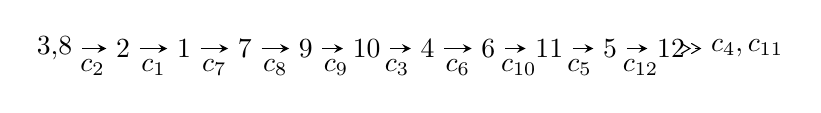
\begin{tikzpicture}[x=22pt, y=7pt]
	% node
	\node (A0) at (-1/8, 0) {3,8};
	\node (A1) at (1, 0) {2};
	\node (A2) at (2, 0) {1};
	\node (A3) at (3, 0) {7};
	\node (A4) at (4, 0) {9};
	\node (A5) at (5, 0) {10};
	\node (A6) at (6, 0) {4};
	\node (A7) at (7, 0) {6};
	\node (A8) at (8, 0) {11};
	\node (A9) at (9, 0) {5};
	\node (A10) at (10, 0) {12};
	\node (C1) at (1/2, -1) {$c_{2}$};
	\node (C2) at (3/2, -1) {$c_{1}$};
	\node (C3) at (5/2, -1) {$c_{7}$};
	\node (C4) at (7/2, -1) {$c_{8}$};
	\node (C5) at (9/2, -1) {$c_{9}$};
	\node (C6) at (11/2, -1) {$c_{3}$};
	\node (C7) at (13/2, -1) {$c_{6}$};
	\node (C8) at (15/2, -1) {$c_{10}$};
	\node (C9) at (17/2, -1) {$c_{5}$};
	\node (C10) at (19/2, -1) {$c_{12}$};
	\node (A11) at (45/4, 0) {$c_{4},c_{11}$};

	% edge
	\draw[->,>=stealth]	
	(A0) edge (A1) (A1) edge (A2) (A2) edge (A3) (A3) edge (A4) (A4) edge (A5) (A5) edge (A6) (A6) edge (A7) (A7) edge (A8) (A8) edge (A9) (A9) edge (A10) ;
	\draw[->>,>={angle 60}]	
	(A10) edge (A11);
\end{tikzpicture} \\ 

\end{tabular} \\

\footnotetext{
The image of knot diagram is generated by the software ``\textbf{Draw programme}" developed by Andrew Bartholomew(\url{http://www.layer8.co.uk/maths/draw/index.htm\#Running-draw}), where we modified some parts for our purpose(\url{https://github.com/CATsTAILs/LinksPainter}).
}\phantom \\ \newline 
\centering \textbf{Ideals for irreducible components\footnotemark of $X_{\text{par}}$} 
 
\begin{align*}
I^u_{1}&=\langle 
u^{44}- u^{43}+\cdots- u^2+1\rangle \\
\\
\end{align*}
\raggedright * 1 irreducible components of $\dim_{\mathbb{C}}=0$, with total 44 representations.\\
\footnotetext{All coefficients of polynomials are rational numbers. But the coefficients are sometimes approximated in decimal forms when there is not enough margin.}
\newpage
\renewcommand{\arraystretch}{1}
\centering \section*{I. $I^u_{1}= \langle u^{44}- u^{43}+\cdots- u^2+1 \rangle$}
\flushleft \textbf{(i) Arc colorings}\\
\begin{tabular}{m{7pt} m{180pt} m{7pt} m{180pt} }
\flushright $a_{3}=$&$\begin{pmatrix}1\\0\end{pmatrix}$ \\
\flushright $a_{8}=$&$\begin{pmatrix}0\\u\end{pmatrix}$ \\
\flushright $a_{2}=$&$\begin{pmatrix}1\\- u^2\end{pmatrix}$ \\
\flushright $a_{1}=$&$\begin{pmatrix}- u^2+1\\- u^2\end{pmatrix}$ \\
\flushright $a_{7}=$&$\begin{pmatrix}u\\- u^3+u\end{pmatrix}$ \\
\flushright $a_{9}=$&$\begin{pmatrix}- u^3\\u^5- u^3+u\end{pmatrix}$ \\
\flushright $a_{10}=$&$\begin{pmatrix}u^9-2 u^7+3 u^5-4 u^3+u\\u^9- u^7+3 u^5-2 u^3+u\end{pmatrix}$ \\
\flushright $a_{4}=$&$\begin{pmatrix}- u^{18}+3 u^{16}-8 u^{14}+15 u^{12}-19 u^{10}+21 u^8-14 u^6+6 u^4- u^2+1\\- u^{18}+2 u^{16}-7 u^{14}+10 u^{12}-15 u^{10}+14 u^8-10 u^6+4 u^4- u^2\end{pmatrix}$ \\
\flushright $a_{6}=$&$\begin{pmatrix}u^5+u\\- u^7+u^5-2 u^3+u\end{pmatrix}$ \\
\flushright $a_{11}=$&$\begin{pmatrix}u^{21}-2 u^{19}+\cdots-4 u^3+u\\- u^{23}+3 u^{21}+\cdots-2 u^3+u\end{pmatrix}$ \\
\flushright $a_{5}=$&$\begin{pmatrix}u^{37}-4 u^{35}+\cdots+5 u^5+u\\- u^{39}+5 u^{37}+\cdots-2 u^3+u\end{pmatrix}$ \\
\flushright $a_{12}=$&$\begin{pmatrix}- u^{34}+5 u^{32}+\cdots- u^2+1\\- u^{34}+4 u^{32}+\cdots-4 u^6- u^2\end{pmatrix}$\\&\end{tabular}
\flushleft \textbf{(ii) Obstruction class $= -1$}\\~\\
\flushleft \textbf{(iii) Cusp Shapes $= 4 u^{43}-24 u^{41}+\cdots-8 u+2$}\\~\\
\newpage\renewcommand{\arraystretch}{1}
\flushleft \textbf{(iv) u-Polynomials at the component}\newline \\
\begin{tabular}{m{50pt}|m{274pt}}
Crossings & \hspace{64pt}u-Polynomials at each crossing \\
\hline $$\begin{aligned}c_{1},c_{6},c_{8}\end{aligned}$$&$\begin{aligned}
&u^{44}+11 u^{43}+\cdots+2 u+1
\end{aligned}$\\
\hline $$\begin{aligned}c_{2},c_{7}\end{aligned}$$&$\begin{aligned}
&u^{44}+u^{43}+\cdots- u^2+1
\end{aligned}$\\
\hline $$\begin{aligned}c_{3}\end{aligned}$$&$\begin{aligned}
&u^{44}+u^{43}+\cdots-20 u+1
\end{aligned}$\\
\hline $$\begin{aligned}c_{4},c_{5},c_{10}\\c_{11},c_{12}\end{aligned}$$&$\begin{aligned}
&u^{44}+u^{43}+\cdots+2 u+1
\end{aligned}$\\
\hline $$\begin{aligned}c_{9}\end{aligned}$$&$\begin{aligned}
&u^{44}-7 u^{43}+\cdots-82 u+7
\end{aligned}$\\
\hline
\end{tabular}\\~\\
\newpage\renewcommand{\arraystretch}{1}
\flushleft \textbf{(v) Riley Polynomials at the component}\newline \\
\begin{tabular}{m{50pt}|m{274pt}}
Crossings & \hspace{64pt}Riley Polynomials at each crossing \\
\hline $$\begin{aligned}c_{1},c_{6},c_{8}\end{aligned}$$&$\begin{aligned}
&y^{44}+45 y^{43}+\cdots+22 y+1
\end{aligned}$\\
\hline $$\begin{aligned}c_{2},c_{7}\end{aligned}$$&$\begin{aligned}
&y^{44}-11 y^{43}+\cdots-2 y+1
\end{aligned}$\\
\hline $$\begin{aligned}c_{3}\end{aligned}$$&$\begin{aligned}
&y^{44}+y^{43}+\cdots-146 y+1
\end{aligned}$\\
\hline $$\begin{aligned}c_{4},c_{5},c_{10}\\c_{11},c_{12}\end{aligned}$$&$\begin{aligned}
&y^{44}+57 y^{43}+\cdots-2 y+1
\end{aligned}$\\
\hline $$\begin{aligned}c_{9}\end{aligned}$$&$\begin{aligned}
&y^{44}+5 y^{43}+\cdots-662 y+49
\end{aligned}$\\
\hline
\end{tabular}\\~\\
\newpage\flushleft \textbf{(vi) Complex Volumes and Cusp Shapes}
$$\begin{array}{c|c|c}  
\text{Solutions to }I^u_{1}& \I (\text{vol} + \sqrt{-1}CS) & \text{Cusp shape}\\
 \hline 
\begin{aligned}
u &= \phantom{-}0.973577 + 0.164922 I\end{aligned}
 & -15.0825 + 1.6902 I & -8.15131 + 0.48221 I \\ \hline\begin{aligned}
u &= \phantom{-}0.973577 - 0.164922 I\end{aligned}
 & -15.0825 - 1.6902 I & -8.15131 - 0.48221 I \\ \hline\begin{aligned}
u &= \phantom{-}0.953126 + 0.350659 I\end{aligned}
 & -4.40949 - 6.07307 I & -4.94666 + 8.49917 I \\ \hline\begin{aligned}
u &= \phantom{-}0.953126 - 0.350659 I\end{aligned}
 & -4.40949 + 6.07307 I & -4.94666 - 8.49917 I \\ \hline\begin{aligned}
u &= -0.895823 + 0.344349 I\end{aligned}
 & -0.76004 + 3.52272 I & \phantom{-}0.90093 - 8.67149 I \\ \hline\begin{aligned}
u &= -0.895823 - 0.344349 I\end{aligned}
 & -0.76004 - 3.52272 I & \phantom{-}0.90093 + 8.67149 I \\ \hline\begin{aligned}
u &= -0.984525 + 0.354824 I\end{aligned}
 & -13.9897 + 7.4569 I & -5.72896 - 6.66961 I \\ \hline\begin{aligned}
u &= -0.984525 - 0.354824 I\end{aligned}
 & -13.9897 - 7.4569 I & -5.72896 + 6.66961 I \\ \hline\begin{aligned}
u &= -0.925891 + 0.175432 I\end{aligned}
 & -5.40173 - 0.74499 I & -8.08077 + 0.34406 I \\ \hline\begin{aligned}
u &= -0.925891 - 0.175432 I\end{aligned}
 & -5.40173 + 0.74499 I & -8.08077 - 0.34406 I \\ \hline\begin{aligned}
u &= \phantom{-}0.827466 + 0.255178 I\end{aligned}
 & -1.38547 - 0.92460 I & -2.73817 + 0.09424 I \\ \hline\begin{aligned}
u &= \phantom{-}0.827466 - 0.255178 I\end{aligned}
 & -1.38547 + 0.92460 I & -2.73817 - 0.09424 I \\ \hline\begin{aligned}
u &= -0.615862 + 0.604835 I\end{aligned}
 & -9.75255 + 2.21449 I & \phantom{-}0.08262 - 3.14030 I \\ \hline\begin{aligned}
u &= -0.615862 - 0.604835 I\end{aligned}
 & -9.75255 - 2.21449 I & \phantom{-}0.08262 + 3.14030 I \\ \hline\begin{aligned}
u &= -0.902990 + 0.718759 I\end{aligned}
 & -10.10340 + 2.72623 I & -2.70072 - 3.12149 I \\ \hline\begin{aligned}
u &= -0.902990 - 0.718759 I\end{aligned}
 & -10.10340 - 2.72623 I & -2.70072 + 3.12149 I \\ \hline\begin{aligned}
u &= \phantom{-}0.892831 + 0.769198 I\end{aligned}
 & -0.21070 - 2.90742 I & -2.24337 + 2.68440 I \\ \hline\begin{aligned}
u &= \phantom{-}0.892831 - 0.769198 I\end{aligned}
 & -0.21070 + 2.90742 I & -2.24337 - 2.68440 I \\ \hline\begin{aligned}
u &= \phantom{-}0.817945 + 0.876060 I\end{aligned}
 & -6.01810 + 5.50586 I & \phantom{-0.000000 } 0. - 1.93289 I \\ \hline\begin{aligned}
u &= \phantom{-}0.817945 - 0.876060 I\end{aligned}
 & -6.01810 - 5.50586 I & \phantom{-0.000000 -}0. + 1.93289 I \\ \hline\begin{aligned}
u &= -0.829954 + 0.866717 I\end{aligned}
 & \phantom{-}3.36907 - 3.82326 I & \phantom{-}1.37231 + 3.41233 I \\ \hline\begin{aligned}
u &= -0.829954 - 0.866717 I\end{aligned}
 & \phantom{-}3.36907 + 3.82326 I & \phantom{-}1.37231 - 3.41233 I \\ \hline\begin{aligned}
u &= \phantom{-}0.848035 + 0.857865 I\end{aligned}
 & \phantom{-}6.75596 + 0.77249 I & \phantom{-}6.88350 - 1.61671 I \\ \hline\begin{aligned}
u &= \phantom{-}0.848035 - 0.857865 I\end{aligned}
 & \phantom{-}6.75596 - 0.77249 I & \phantom{-}6.88350 + 1.61671 I \\ \hline\begin{aligned}
u &= -0.869487 + 0.843192 I\end{aligned}
 & \phantom{-}5.36576 + 2.39601 I & \phantom{-}3.40471 - 4.61138 I \\ \hline\begin{aligned}
u &= -0.869487 - 0.843192 I\end{aligned}
 & \phantom{-}5.36576 - 2.39601 I & \phantom{-}3.40471 + 4.61138 I \\ \hline\begin{aligned}
u &= -0.932920 + 0.818861 I\end{aligned}
 & \phantom{-}5.16549 + 3.79714 I & \phantom{-}3.00062 + 0. I\phantom{ +0.000000I} \\ \hline\begin{aligned}
u &= -0.932920 - 0.818861 I\end{aligned}
 & \phantom{-}5.16549 - 3.79714 I & \phantom{-}3.00062 + 0. I\phantom{ +0.000000I} \\ \hline\begin{aligned}
u &= \phantom{-}0.909164 + 0.854591 I\end{aligned}
 & -2.08909 - 3.16925 I & \phantom{-}2.00000 + 2.55615 I \\ \hline\begin{aligned}
u &= \phantom{-}0.909164 - 0.854591 I\end{aligned}
 & -2.08909 + 3.16925 I & \phantom{-}2.00000 - 2.55615 I\\
 \hline 
 \end{array}$$\newpage$$\begin{array}{c|c|c}  
\text{Solutions to }I^u_{1}& \I (\text{vol} + \sqrt{-1}CS) & \text{Cusp shape}\\
 \hline 
\begin{aligned}
u &= \phantom{-}0.954586 + 0.818188 I\end{aligned}
 & \phantom{-}6.42188 - 7.00665 I & \phantom{-}5.98798 + 6.76938 I \\ \hline\begin{aligned}
u &= \phantom{-}0.954586 - 0.818188 I\end{aligned}
 & \phantom{-}6.42188 + 7.00665 I & \phantom{-}5.98798 - 6.76938 I \\ \hline\begin{aligned}
u &= -0.969590 + 0.814117 I\end{aligned}
 & \phantom{-}2.93183 + 10.06920 I & \phantom{-0.000000 } 0. - 8.25971 I \\ \hline\begin{aligned}
u &= -0.969590 - 0.814117 I\end{aligned}
 & \phantom{-}2.93183 - 10.06920 I & \phantom{-0.000000 -}0. + 8.25971 I \\ \hline\begin{aligned}
u &= \phantom{-}0.980677 + 0.812716 I\end{aligned}
 & -6.52850 - 11.77360 I & \phantom{-0.000000 -}0. + 6.74145 I \\ \hline\begin{aligned}
u &= \phantom{-}0.980677 - 0.812716 I\end{aligned}
 & -6.52850 + 11.77360 I & \phantom{-0.000000 } 0. - 6.74145 I \\ \hline\begin{aligned}
u &= \phantom{-}0.554006 + 0.459665 I\end{aligned}
 & -0.93127 - 1.66423 I & \phantom{-}1.39492 + 5.36634 I \\ \hline\begin{aligned}
u &= \phantom{-}0.554006 - 0.459665 I\end{aligned}
 & -0.93127 + 1.66423 I & \phantom{-}1.39492 - 5.36634 I \\ \hline\begin{aligned}
u &= -0.177999 + 0.637957 I\end{aligned}
 & -11.46970 - 3.90382 I & -0.05667 + 2.21807 I \\ \hline\begin{aligned}
u &= -0.177999 - 0.637957 I\end{aligned}
 & -11.46970 + 3.90382 I & -0.05667 - 2.21807 I \\ \hline\begin{aligned}
u &= \phantom{-}0.196554 + 0.570963 I\end{aligned}
 & -2.11354 + 2.70365 I & \phantom{-}0.96683 - 3.89024 I \\ \hline\begin{aligned}
u &= \phantom{-}0.196554 - 0.570963 I\end{aligned}
 & -2.11354 - 2.70365 I & \phantom{-}0.96683 + 3.89024 I \\ \hline\begin{aligned}
u &= -0.302925 + 0.453673 I\end{aligned}
 & \phantom{-}1.018180 - 0.410960 I & \phantom{-}9.05285 + 1.73879 I \\ \hline\begin{aligned}
u &= -0.302925 - 0.453673 I\end{aligned}
 & \phantom{-}1.018180 + 0.410960 I & \phantom{-}9.05285 - 1.73879 I\\
 \hline 
 \end{array}$$\newpage
\newpage\renewcommand{\arraystretch}{1}
\centering \section*{ II. u-Polynomials}
\begin{tabular}{m{50pt}|m{274pt}}
Crossings & \hspace{64pt}u-Polynomials at each crossing \\
\hline $$\begin{aligned}c_{1},c_{6},c_{8}\end{aligned}$$&$\begin{aligned}
&u^{44}+11 u^{43}+\cdots+2 u+1
\end{aligned}$\\
\hline $$\begin{aligned}c_{2},c_{7}\end{aligned}$$&$\begin{aligned}
&u^{44}+u^{43}+\cdots- u^2+1
\end{aligned}$\\
\hline $$\begin{aligned}c_{3}\end{aligned}$$&$\begin{aligned}
&u^{44}+u^{43}+\cdots-20 u+1
\end{aligned}$\\
\hline $$\begin{aligned}c_{4},c_{5},c_{10}\\c_{11},c_{12}\end{aligned}$$&$\begin{aligned}
&u^{44}+u^{43}+\cdots+2 u+1
\end{aligned}$\\
\hline $$\begin{aligned}c_{9}\end{aligned}$$&$\begin{aligned}
&u^{44}-7 u^{43}+\cdots-82 u+7
\end{aligned}$\\
\hline
\end{tabular}\newpage\renewcommand{\arraystretch}{1}
\centering \section*{ III. Riley Polynomials}
\begin{tabular}{m{50pt}|m{274pt}}
Crossings & \hspace{64pt}Riley Polynomials at each crossing \\
\hline $$\begin{aligned}c_{1},c_{6},c_{8}\end{aligned}$$&$\begin{aligned}
&y^{44}+45 y^{43}+\cdots+22 y+1
\end{aligned}$\\
\hline $$\begin{aligned}c_{2},c_{7}\end{aligned}$$&$\begin{aligned}
&y^{44}-11 y^{43}+\cdots-2 y+1
\end{aligned}$\\
\hline $$\begin{aligned}c_{3}\end{aligned}$$&$\begin{aligned}
&y^{44}+y^{43}+\cdots-146 y+1
\end{aligned}$\\
\hline $$\begin{aligned}c_{4},c_{5},c_{10}\\c_{11},c_{12}\end{aligned}$$&$\begin{aligned}
&y^{44}+57 y^{43}+\cdots-2 y+1
\end{aligned}$\\
\hline $$\begin{aligned}c_{9}\end{aligned}$$&$\begin{aligned}
&y^{44}+5 y^{43}+\cdots-662 y+49
\end{aligned}$\\
\hline
\end{tabular}
\vskip 2pc
\end{document}